\documentclass{IEEEcsmag}

\usepackage[colorlinks,urlcolor=blue,linkcolor=blue,citecolor=blue]{hyperref}

\usepackage{upmath}
\usepackage{amssymb}
\usepackage{amsmath}
\usepackage{array}
\newcolumntype{P}[1]{>{\centering\arraybackslash}p{#1}}

\jvol{XX}
\jnum{XX}
\paper{8}
\jmonth{May/June}
\jname{Computing in Science and Engineering}
\pubyear{2021}
\newtheorem{theorem}{Theorem}
\newtheorem{lemma}{Lemma}

\setcounter{secnumdepth}{0}

\begin{document}

\sptitle{Department: Head}
\editor{Editor: Name, xxxx@email}

\title{PyExaFMM: Designing a high-performance particle fast multipole solver in Python with Numba}

\author{S. Kailasa}
\affil{Department of Mathematics, University College London}

\author{T. Wang}
\affil{Department of Mechanical and Aerospace Engineering, The George Washington University}

\author{\text{L}. A. Barba}
\affil{Department of Mechanical and Aerospace Engineering, The George Washington University}

\author{T. Betcke}
\affil{Department of Mathematics, University College London}

\markboth{Department Head}{Paper title}

\begin{abstract}
The particle fast multipole method is a good case study for understanding the efficacy of Python for developing high-performance software for non-trivial algorithms, due its reliance on a hierarchical tree data structure. In this paper we describe the mathematical and software engineering techniques used to extract performance for PyExaFMM, a Python based solver for the particle fast multipole method, accelerated with Numba, designed to be run on single-node multicore architectures. We report that we achieve runtimes within $\mathcal{O}(10)$ of the state of the art C++ implementation, with comparable accuracy and memory footprint for three dimensional problems in double precision.
\end{abstract}

\maketitle
\chapterinitial{CPython is the original and most} popular implementation of the highly productive, dynamically typed and interpreted, Python programming language, and is written in C. CPython was designed with safety and developer productivity in mind, rather than high-performance computing [HPC]. Pythons's dynamic typing forces objects to be passed through an interpreter loop at runtime, and applications are restricted to a single thread via a `global interpreter lock' [GIL] to ensure thread safety. However, Python's popularity has lead to the development of numerous open-source tools for HPC with CPython, that allow users to bypass the interpreter, develop multithreaded applications, and even deploy source code written in Python to GPUs.

PyExaFMM\footnote{https://www.github.com/exafmm/pyexafmm} is a solver for the three-dimensional particle fast multipole method [FMM], designed to be run on single-node multicore architectures. It was designed to test the efficacy of Numba, a `just-in-time' [JIT] compiler, for developing HPC applications in CPython. Building on the success of the ExaFMM project's comparable C++ implementation \cite{Wang2021}, we wanted to test whether we could retain the productivity benefits of working in Python while achieving performance comparable to compiled languages.  The FMM consists of a recursive loop through a hierarchical data structure. Representing computations and data efficiently while retaining performance is challenging, therefore it offers a good benchmark for studying the efficacy of Python and Numba for developing efficient software for complex algorithms.

Numba appears to offer excellent tools for overcoming the performance problems of Python. It bypasses the interpreter for operations involving loops over Numpy arrays and numeric scalars, translating Python source code into efficient platform-dependent machine code using the LLVM infrastructure. LLVM applies hardware dependent optimizations such as single-instruction multiple data [SIMD] vectorization over loops, to the intermediate bytecode representation [IR] produced by Numba. Bypassing the Python interpreter in this way can make Numba compiled functions competitive with compiled languages such as C++ and Fortran. However, we note that Numba is not able to map all operations specified in Python to efficient machine instructions, or vectorize loops, if they contain operations outside of the subset of numeric Python it optimizes for. Furthermore, Numba still requires interaction with the Python interpreter to pass data to Numba compiled functions, as well as to interact with non-optimized parts of the codebase involved in data-organization or calls to incompatible libraries. Therefore, developers have to be careful to organize their code in such a way as to restrict interaction with the Python interpreter, as well as ensure that their source code can be optimized by Numba, to ensure that they experience a performance benefit from using it.

Numba is a `drop-in' tool. Functions or classes are marked for JIT compilation with a decorator, and `polymorphic dispatching' picks up input and output type data from the objects arguments at runtime - compiling the machine-code for the function for this type signature if it does not already exist in cache. The function itself is called from a Python wrapper which forms the interface between the Python runtime and a Numba compiled function. Therefore Numba fits easily into existing Python projects. Numba has been extended with efficient implementations of many of the array manipulation and linear algebra operations offered by Numpy, as well as multithreading functionality via iterations over a parallel range iterator, reminiscent of OpenMP's parallel for loops. Furthermore, Numba supports the writing of Python kernels for AMD and NVidia GPUS, and is fully integrated with the CuPy library.

Numba therefore provides a `framework' for developing heterogenous, cross-platform, applications using only Python source code. Numba's framework impacts the design of HPC software as performance is dictated by the interaction between the Python interpreter and Numba optimized functions. Developers have to be careful to design Numba functions that are vectorizable, and multithreaded functions that are cache-optimal. Furthermore, care has to be taken to design robust software that limits usage of the Python objects, and instead designs operations in a `data-centric' manner, around Numpy arrays. In this paper we begin by briefly summarizing the kernel independent FMM [KIFMM] algorithm used by PyExaFMM, before proceeding to describe the mathematical optimizations, and software design strategies we used for achieving performance with Numba. We discuss in detail how we parallelize FMM operations to maximize cache-reuse, our approach to designing functions for Numba compilation, as well as how we architected PyExaFMM to minimize interactions between Numba compiled functions and the Python interpreter. We conclude with benchmarks comparing the memory usage, runtimes and accuracy of the software with respect to the comparable state-of-the-art C++ implementation from the ExaFMM project, ExaFMM-T \cite{Wang2021}.

\section{THE FAST MULTIPOLE METHOD}

The particle FMM \cite{Greengard1987} is an algorithm for approximating the $N$-body problem, in which one aims to calculate the pairwise interactions between $N$ particles. Consider a problem domain $ D \subset \mathbb{R}^3$, containing a set of `source' particles at positions $x_i$, and their interaction with a `target' particle at position $y_j$ where $i \in [1,...,N]$, where $x_i, y_j \in \mathbb{R}^3$. The pairwise interaction of the target with all sources can be written as,

\begin{flalign}
	\label{eq:n_body_problem}
	\phi_j = \sum_{i=1}^{N}K(x_i, y_j)q_i
\end{flalign}

where $K(., .)$ is called the `kernel' or Green's function, and the interactions are weighted by $q_i$. This calculation appears in numerous contexts across science and engineering. For example, if we interpret $q_i$ as a charge, and take the Green's function to be,

\begin{flalign}
	K(x, y) = \frac{1}{4\pi|x-y|}
	\label{eq:laplace_kernel}
\end{flalign}

we recognize (\ref{eq:n_body_problem}) as the calculation of the electrostatic potential $\phi_j$ at $y_j$ due to source particles at positions $x_i$ with charges $q_i$. Without loss of generality we can consider the sources and targets to correspond to the same set of particles, we take this as our benchmark problem. A naive calculation of (\ref{eq:n_body_problem}) at $N$ target positions results in an algorithm of $\mathcal{O}(N^2)$ runtime. The FMM is able to approximate this in $\mathcal{O}(N)$, with proscribed error bounds. It works by partitioning $D$ using a hierarchical tree. Level $0$ of the tree corresponds to a cubic box containing all source and target particles, it is then recursively partitioned into $8^l$ boxes where $l$ is a given level. The maximum level $l$, or \textit{leaf level}, of partitioning in a subset of $D$ is set by a user defined constant for the maximum number of particles allowed in a given tree node. Refinement proceeds until this condition is satisfied. Optionally, the domain can be refined in a \textit{non-uniform} manner such that the leaf level consists of boxes of different sizes, reflecting non-uniform particle distributions. Figure (\ref{fig:algorithm}b) illustrates the relationship between a given leaf box $T$ and its neighbors, termed \textit{interaction lists}, for a non-uniform tree in $\mathbb{R}^2$. The $U$ list consists boxes adjacent to $T$ - i.e. sharing an edge or vertex (or face in $\mathbb{R}^3$), known as its \textit{neighbors}. Neighbors at the same level of discretization are known as \textit{colleagues}.  The $V$ list consists of child boxes of the colleagues of $T$'s parent box, which are not-adjacent to $T$. The $W$ list consists of child boxes of $T$'s colleagues, which are not-adjacent to $T$, and the $X$ list consists of boxes for which $T$ is in the $W$ list. The $X$ and $W$ lists only occur in non-uniform trees, are only formed for leaf boxes.

The FMM consists of six operators: P2M, M2M, M2L, L2L, L2P and P2P, where a given operator is read as `X to Y'. `P' stands for particle(s), `M' for multipole expansion and `L' for local expansion. The operators can be seen to correspond to translations between expansion representations. A multipole expansion represents the aggregation of charge located within a given box in the tree, where the expansion center is set to coincide with the box center, and can be truncated to an `expansion order', $p$, for tunable accuracy. A multipole expansion can be translated into a local expansion centered on another box, inside of which it is valid, and it represents the aggregation of charge corresponding to the multipole expansion. This is the M2L operator. Similarly the expansion centers of local or multipole expansions can be shifted, which are the L2L and M2M operators respectively. The P2M operator is the act of forming a multipole expansion for a set of particles. L2P and P2P refer to direct evaluations using (\ref{eq:n_body_problem}) between local expansion coefficients, or source particles, with a set of target particles, respectively.

Figure (\ref{fig:algorithm}) illustrates the FMM for a problem in $\mathbb{R}^2$. Figure (\ref{fig:algorithm}a) shows the recursive partition, and the first step of the algorithm - the \textit{upward pass}. The tree is traversed bottom-up, in which multipole expansions are found for boxes at the leaf level (P2M), the centers of which are shifted to the center of the corresponding `parent box' (M2M) and expansion coefficients summed in order to find the parent's multipole expansion. Figure (\ref{fig:algorithm}c) and Figure (\ref{fig:algorithm}d) show the second step - the \textit{downward pass}. The tree is traversed top-down, starting at level $2$. M2L transfers for nodes in a box's $V$ list are performed, followed by L2L transfers. Resulting in the local expansion for each leaf box. These local expansions compress the far field component of potential for targets within a given leaf, and are evaluated directly at the target particles (L2P). The far field is defined by a box and its ancestors' $V$ lists. The near field, defined by its $U$, $W$ and $X$ lists, is evaluated directly for boxes at the leaf level (P2P). For non-uniform trees the P2P step can be made more efficient by taking advantage of the $X$ and $W$ lists. Consider a leaf box $T$, we can use the multipole expansion of boxes in its $W$ list to evaluate their contribution towards potential for target points in $T$ (M2P). For boxes in $T$'s $X$ list, we can evaluate the source charges directly at the points supporting the local expansion (S2L), before performing L2P.

As we traverse down the tree in the downward pass, more and more of the far field contribution to potential is compressed in the local expansion for a given box. We find this far field component by performing M2L transfers for a given box, over its $V$ list, the size of which is bounded by a constant. Therefore we see the complexity of the FMM to be dictated by the number of nodes in the tree, which due to the maximum particle per node constraint will be restricted to $\mathcal{O}(N)$.

In the KIFMM \cite{Ying2004}, we use evaluations of the kernel function, rather than analytic expansions, to find the multipole and local expansions and translate between them. Consider the P2M operator for a given box illustrated in figure (\ref{fig:operators}a). The multipole expansion is described by equivalent charges placed at $n$ quadrature points evenly spaced on an \textit{equivalent surface} enclosing the box. Where $n$ is related to the expansion order $p$ by,

\begin{flalign}
	n = 6(p-1)^2+2
	\label{eq:order}
\end{flalign}

The sum (\ref{eq:n_body_problem}), for these equivalent charges is matched to the \textit{check potential} $\phi^c$ calculated from the charges in the box directly at quadrature points on a \textit{check surface} that encloses the equivalent surface and the box. Each component of $\phi^c$, corresponding to a point on the check surface $y_j$, is calculated as,

\begin{flalign}
	\phi_{j}^c = \sum_{i=1}^{N_{box}} K(x_i, y_j) q_i
\end{flalign}

where there at most $N_{box}$ particles in the box, with charges $q_i$ and at positions $x_i$. We find the equivalent charges $q^e_i$ corresponding to points $x_i$ on the equivalent surface with,

\begin{flalign}
	\sum_{i=1}^{N_{e}} K(x_i, y_j)q^e_i = \phi^c
\end{flalign}

Where $N_e$ is the number of quadrature points on the equivalent surface. In matrix form,

\begin{flalign}
	K q_{e} = \phi^c \\
	q_e = K^{-1} \phi^c
	\label{eq:p2m}
\end{flalign}

The matrix on the right hand side of (\ref{eq:p2m}) is taken to be the P2M operator. This logic is repeated to form the other KIFMM operators, the required check and equivalent surfaces and matchings are illustrated in figure (\ref{fig:operators}). We note that for the L2L and M2L operators, the equivalent surface around the target box encloses the check surface, which itself encloses the target box. This is reflective of the region of validity of local expansions. The check potentials are then formed with the child/parent equivalent charges for the M2M and L2L operators respectively, and with the equivalent charges of boxes in the $V$ list of a given box, for its corresponding M2L operator. The L2P, M2P, S2L and P2P operators are evaluated directly using (\ref{eq:n_body_problem}). We note that large values of $p$ lead to poor conditioning in the inversion of the matrix $K$, and in practice we solve this by taking the \textit{backward-stable pseudo-inverse} of $K$, introduced by Malhotra et. al \cite{Malhotra2015}.

% Larger figure
\begin{figure*}
	\centerline{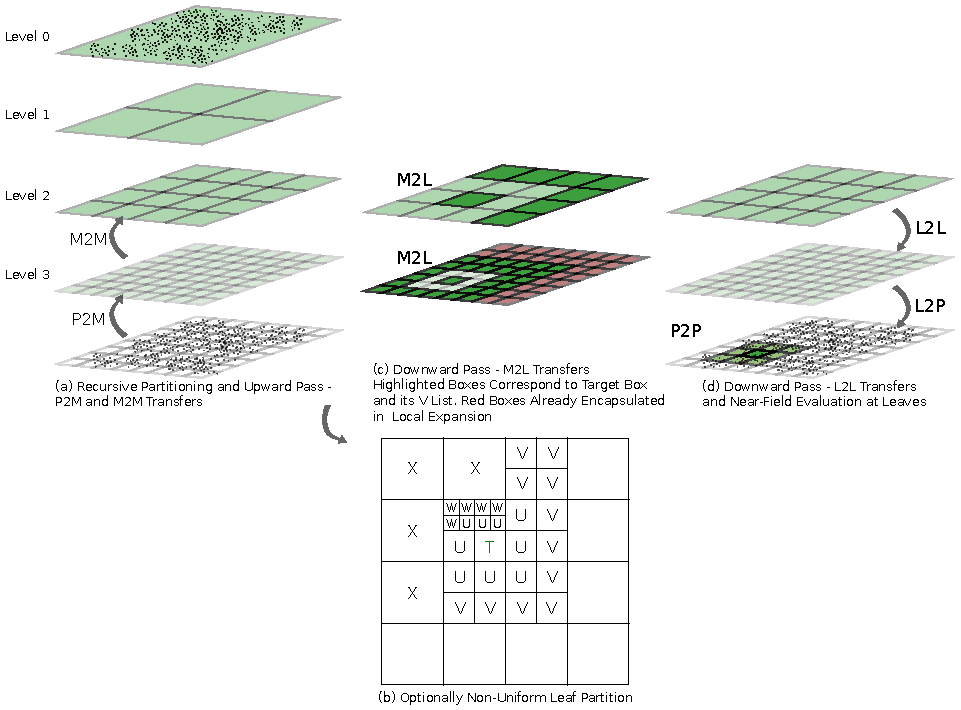
\includegraphics {figures/tree.pdf}}
	\caption{FMM algorithm and operator actions, including tree construction, illustrated for problem in $\mathbb{R}^2$.}
	\label{fig:algorithm}
\end{figure*}

\begin{figure*}
	\centerline{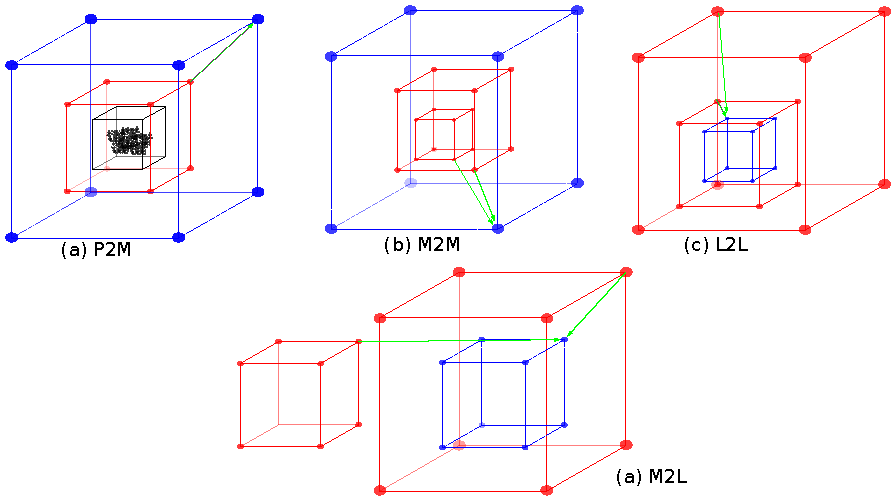
\includegraphics {figures/operators.pdf}}
	\caption{KIFMM operator calculations for order $p=2$ expansions. Equivalent charges placed at quadrature points on the (red) equivalent surfaces, are matched at quadrature points on the (blue) check surfaces. Charges are plotted in black, and green arrows are used to indicate least-squares fittings.}
	\label{fig:operators}
\end{figure*}


\section{TECHNIQUES FOR ACHIEVING PERFORMANCE}

\subsection{Compressing M2L Operator with SVD}

The maximum size of a $V$ list in three dimensions is 189. Therefore naively forming M2L matrices, and performing inversions for each box during the downward pass is costly. Instead, we label each unique $V$ list interaction at a given tree level with a \textit{transfer vector} \cite{Fong2009}. Note that there are at most $7^3-3^3=316$ transfer vectors at a given level. As usual we seek the equivalent charge around a target box due to a source box in its $V$ list, by matching the kernel evaluations at a check surface enclosing the target box and its equivalent surface,

\begin{flalign}
	K^{se2tc} q^s_e = K^{te2tc} q^t_e
\end{flalign}

where $K^{se2tc}$ is the matrix with elements calculated using (\ref{eq:laplace_kernel}), between the source box's equivalent surface, and a target box's check surface, $K^{te2tc}$ is calculated using the target box's equivalent and check surfaces, $q^s_e$ is the known equivalent charge at the source box, and $q^t_e$ is unknown. We form the M2L matrix by inverting $K^{te2tc}$,

\begin{flalign}
	q^t_e = \underbrace{(K^{te2tc})^{-1} K^{se2tc}}_{M2L} q^s_e
\end{flalign}

We can form an M2L matrix at level $l$, for source boxes corresponding to all unique transfer vectors for a single target box, and concatenate them,

\begin{flalign}
	M2L_{l} = \begin{pmatrix}
M2L_1 & M2L_2 & ... &  M2L_{316}
\label{eq:concatenated_m2l}
\end{pmatrix}
\end{flalign}

Note that $M2L_l \in \mathbb{R}^{N_c \times 316N_e}$, where $N_c$ and $N_e$ are the number of quadrature points on the check and equivalent surfaces, respectively. When we encounter an M2L interaction during the downward pass, we simply compute the corresponding transfer vector and lookup the sub-matrix of (\ref{eq:concatenated_m2l}), which can be pre-computed and cached, that corresponds to its M2L matrix. PyExaFMM reduces the application and storage costs of concatenated M2L matrices for a given level further by applying \textit{SVD compression} to (\ref{eq:concatenated_m2l}). Consider taking the SVD of $M2L_l$

\begin{flalign}
	M2L_l = \sum_{j=1}^r \sigma_ju_jv_j^T
\end{flalign}

where $r=\text{rank}(M2L_l) = N_c$ is the row rank, $u_j$ and $v_j$ are the left and right singular vectors respectively, and the singular values $\sigma_j$ are arranged in weakly decreasing order. We can cutoff this sum at a \textit{compression rank} $k \leq N_c$ to approximate $M2L_l$. PyExaFMM implements the \textit{randomized SVD} of Halko et. al \cite{Halko2011}. The algorithm can be decomposed into a series of matrix vector products, optimized by BLAS, making it fast to compute.

\subsection{Software Design}

- (1) Function composition. PyExaFMM consists of (compositions of) simple functions that make use of: bitwise operations, simple arithmetic. Example of Morton encoding functions, and how we don't pay further cost for passing into Numba once already there. Describe how parametrization of operators works in PyExaFMM (i.e. how data is copied to operators and the relative costs involved). Should mention that tree building library is separated from FMM library.


- (2) Data oriented programming and API. API exposed via FMM class is a thin wrapper around numpy arrays containing expansion coefficients, potentials/gradients, and particle positions/charges. FMM loop logic is coded in Python, however actual floating point operations take place in numba compiled functions - separated via a `backend' interface. Storage of coefficients and results in vectors. Lookup tables for indices.

- (2') Architecture of library with reference to UML diagram and composition idea. i.e. start of with simple functions, create more complex Numba compiled operator functions, these are then alled from the thin Python layer.

- (3) Operator and tree precomputations. Technology used (HDF5). User configuration for experiments.

- (4) Conciseness of library. Python's expressiveness allows PyExaFMM to be a concise library, consisting of $\sim$3,000 lines of code, in comparison to comparable single-node C++ implementations ExaFMM-T ($\sim$7000 lines) \cite{Wang2021} or TBFMM ($\sim$20,000) \cite{Bramas2020}. This makes it easy for domain specialists to hack for their needs, without having to traverse a large/complex codebase.

% Larger figure
\begin{figure*}
	\centerline{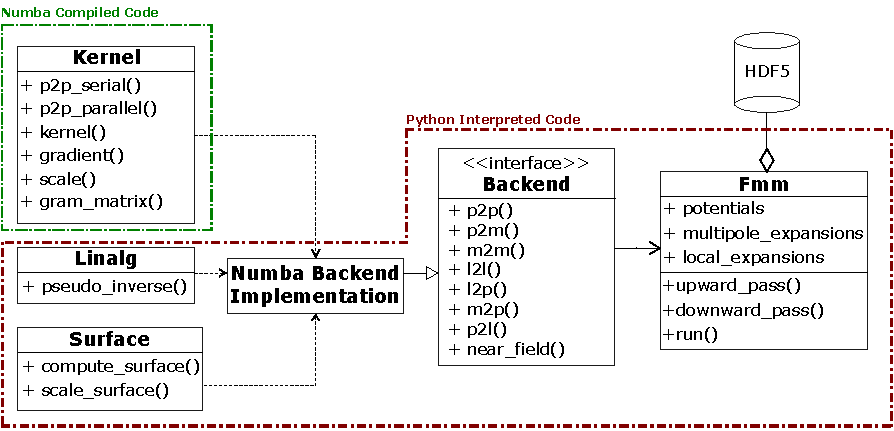
\includegraphics {figures/software.pdf}}
	\caption{Simplified UML model of all PyExaFMM components. Trees and operators are precomputed and stored in the HDF5 database. Except for the `Fmm' object which acts as the user interface, all other components are modules consisting of simple functions.}
	\label{fig:design}
\end{figure*}

\subsection{Parallelization Strategies for FMM operators}

- (0) Carefully set threading layer/settings of Numba.

- (1) Allocate memory (if possible) aligning targets/sources - and run kernel function over them. Maximizes cache re-use (P2M, L2P, Near Field)

- (2) Simple parallel for loop over interactions - S2L (not enough computation for it to be worth it) M2T (too expensive)

- (3) Threads restricted to simple blas l3 operations and lookups, except M2L operator. This requires more than simple lookup. Comment on need for fast hash function compatible with Numba. Comment on how this is (a) an example of function composition of simple functions (b) an example of a potential pitfall for naive users, and will lead to slow performance if you use a native hashing function.

\section{Benchmarks}

- (0) Mention machine used for computing benchmarks. Offer time benchmark for pre-computations wrt to C++ (trees + operators).

- (1) Mention that C++ lib doesn't do M2L compression, instead does FFT based convolution.

- (2) Comment on fractional runtimes of operators. Relative impact of compression (minimal), and how this shows that the complexity of the two softwares must be similar, and that the difference must be explained due to the Python/Numba interface.

% Smaller figure
\begin{figure}
	\centerline{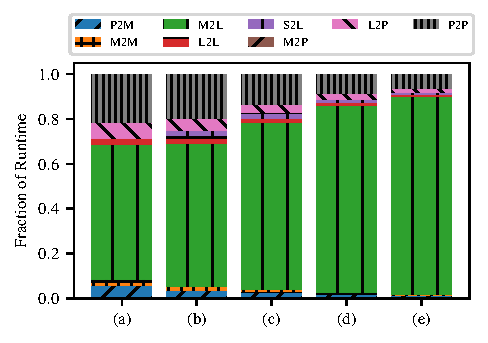
\includegraphics {figures/operator_runtimes.pdf}}
	\caption{Foo bar}
	\label{fig:operator_runtimes}
\end{figure}

\begin{table*}
	\centering
	\caption{Relative error, runtime and peak memory consumption in comparison to the SOTA. Experiments run with $N=1,000,000$ points tested in two geometries: (1) distributed randomly in a cubic unit box, (2) distributed randomly on the surface of a sphere with unit radius, leading to $M$ leaves in their respective geometries, with a maximum of $150$ points per leaf, multipole and local expansions of order $p$, and a compression rank $k$ for PyExaFMM. Charge densities are chosen in the interval $[0, 1)$. Runtimes exclude tree building time. Reported to 3 significant figures after a single run.}
	\begin{tabular}{|*{10}{c|}}
		\hline
		& & &   & \multicolumn{2}{c|}{Runtime} & \multicolumn{2}{c|}{Peak Memory} & \multicolumn{2}{c|}{Relative Error}\\
		\hline
		$k$ & $M$ &$p$ &  Geometry   &   PyExaFMM  &  ExaFMM-T &    PyExaFMM  &  ExaFMM-T  &   PyExaFMM  &  ExaFMM-T\\
		\hline
		10 & 17,017 & 6   &   Sphere  &  $10.6 \pm 0.1$ s & $0.41 \pm 0.04$ s  &  2.96 GB  &   2.34 GB  & 1.00e-4 & 8.75e-5\\
		 & 32,768 &    &   Random  &  $13.2 \pm 0.2$ s &  $0.41 \pm 0.05$ s &  4.93 GB  &   2.98 GB  & 8.75e-5 & 7.66e-5\\
		 &  & 10   &   Sphere  &  $57.0 \pm 0.1$ s &  $1.78 \pm 0.04$ s  &  3.09 GB  &   3.22 GB  & 2.00e-6 & 2.86e-6\\
		 &  &    &   Random  & $131 \pm 2$ s &   $2.11 \pm 0.06$ s  &  4.93 GB  &   3.88 GB  & 1.71e-6 & 3.84e-6\\
%%%%
		100 & 17,017 & 6   &   Sphere  &  $10.6 \pm 0.1$ s & $0.41 \pm 0.04$ s  &  2.96 GB  &   2.34 GB  & 1.00e-4 & 8.75e-5\\
		 & 32,768 &    &   Random  &  $13.2 \pm 0.2$ s &  $0.41 \pm 0.05$ s &  4.93 GB  &   2.98 GB  & 8.75e-5 & 7.66e-5\\
		 &  & 10   &   Sphere  &  $57.0 \pm 0.1$ s &  $1.78 \pm 0.04$ s  &  3.09 GB  &   3.22 GB  & 2.00e-6 & 2.86e-6\\
		 &  &    &   Random  & $131 \pm 2$ s &   $2.11 \pm 0.06$ s  &  4.93 GB  &   3.88 GB  & 1.71e-6 & 3.84e-6\\
%%%%
		Full Rank & 17,017 & 6   &   Sphere  &  $10.6 \pm 0.1$ s & $0.41 \pm 0.04$ s  &  2.96 GB  &   2.34 GB  & 1.00e-4 & 8.75e-5\\
		 & 32,768 &    &   Random  &  $13.2 \pm 0.2$ s &  $0.41 \pm 0.05$ s &  4.93 GB  &   2.98 GB  & 8.75e-5 & 7.66e-5\\
		 &  & 10   &   Sphere  &  $57.0 \pm 0.1$ s &  $1.78 \pm 0.04$ s  &  3.09 GB  &   3.22 GB  & 2.00e-6 & 2.86e-6\\
		 &  &    &   Random  & $131 \pm 2$ s &   $2.11 \pm 0.06$ s  &  4.93 GB  &   3.88 GB  & 1.71e-6 & 3.84e-6\\
		\hline
	\end{tabular}
	\label{tab:performance}
 \end{table*}


\section{CONCLUSION}

- Numba constraints software design, and has its own learning curve. Not simple to just drop in and expect performance boost.

- Performance debugging for more complex applications requires more knowledge than novice users can be expected to have.

- Numba doesn't help much if there are big interpreter related costs (using large Numpy arrays) which add a large constant to runtime complexity.

- Numba is clearly insufficient for more complex HPC applications, however performance is still fairly remarkable. Not to mention other benefits of Numba (rapid prototyping with Python, cross-platform builds, GPU development etc.)


\section{ACKNOWLEDGMENT}

SK is supported by EPSRC Studentship 2417009.

\bibliography{pyexafmm}

\bibliographystyle{ieeetr}

\begin{IEEEbiography}{Srinath Kailasa}{\,}is a Graduate Student at UCL, currently pursuing a PhD in Computational Mathematics. He completed an MPhys in Physics (2017) and an MSc in Scientific Computing (2020) from Durham University and UCL respectively, interspersed with time as a Software Engineer in industry. His research interests are in high-performance and scientific computing. Contact him at srinath.kailasa.18@ucl.ac.uk.
\end{IEEEbiography}

\begin{IEEEbiography}{Tingyu Wang}{\,}is a PhD student in Mechanical Engineering at the George Washington University. Contact him at twang66@email.gwu.edu.
\end{IEEEbiography}

\begin{IEEEbiography}{Lorena. A. Barba}{\,}is a Professor of Mechanical and Aerospace Engineering at the George Washington University.  Contact her at labarba@email.gwu.edu.
\end{IEEEbiography}

\begin{IEEEbiography}{Timo Betcke}{\,}is Professor of Computational Mathematics at University College London. Is the lead investigator of the Bempp project, an open-source boundary element library. He studied Engineering in Germany as Undergraduate and then completed a PhD in Oxford in Numerical Analysis. From 2005 to 2006 he had various research positions until he became a Lecturer at UCL in 2011. Since 2018 he is a full Professor in the Department of Mathematics at UCL. Contact him at t.betcke@ucl.ac.uk.
\end{IEEEbiography}
\end{document}

